%!TEX root = ../physical-olympics-2.tex
\chapter{静磁学} 


\section{电流与磁场}

\subsection{磁场地位与电流分布}

在历史上很长一段时期内, 磁学与电学的研究一直彼此独立地发展着. 丹麦物理学家\emph{奥斯特}({\it H. C.\O rsted})多年的研究成果在1819-1820陆续地发表使得主流科学家们认识到电与磁之间的联系. 从此电磁学的发展进入一个新的时期. 人们对磁的认识一共经历了几个阶段:
\begin{enumerate}
\item 萌芽阶段: 奥斯特之前的阶段. 磁现象被认为与\emph{磁体}(magnet), 主要是四氧化三铁为主要成分的矿石相关. 它被设想为与电现象的电荷类似的\emph{磁荷}(magnetic charge)造成的现象, 也是平方反比的纵向力. 偶尔有记录电击导致材料磁化的现象.
\item 唯象阶段: 奥斯特到\emph{麦克斯韦}({\it J. C. Maxwell})之间的阶段. 人们普遍认识到电与磁之间的联系, 电流也会产生磁效应, 得益于\emph{法拉第}({\it M. Faraday})与\emph{亨利}{\it J. Henry}, 人们一方面建立了``场''的观念, 另一方面也发现与描述了磁场变化造成的电效应. 而\emph{安培}({\it A.-M. Amp\`ere})等人的工作定量地描述了电流产生的磁场, 它是一种新奇的横向力. 安培的\emph{分子电流假说}解释了磁铁的磁性本质上就是分子电流产生磁场的结果.
\item 本质阶段: 麦克斯韦到\emph{狄拉克}({\it P. Dirac})之间的阶段. 人们发现电流的本质是运动的电荷. 从而磁场的概念被进一步修正为: 运动电荷之间的相互作用. 麦克斯韦和\emph{洛伦兹}({\it H. A. Lorentz})给出了电磁场的普遍理论, 即\emph{电动力学}(electrodynamics)\footnote{这个词语却是安培发明的.}, 发现了磁场不过是电场的相对论产物. \emph{赫兹}({\it H. R. Hertz})的实验有效地支持了电磁场论. 同时微观粒子的陆续发现伴随着人们对物质本质的研究进入了量子时代, 电子的\emph{自旋}(spin)与\emph{磁矩}(magnetic moment)被发现与研究.
\item 现代阶段: 狄拉克之后的阶段. 狄拉克提出了\emph{量子电动力学}(quantum electrodynamics), 主张把电子也作为一个类似于电磁场的场, 与电磁场作为整体来研究各自的规律和其相互作用. 成功解释了电子的自旋, 预言了反物质的存在并被实验证实. 提出了\emph{磁单极子}(magnetic monopole)的模型. 相关的研究持续至今.
\end{enumerate}

现在, 我们对\emph{磁场}(magnetic field)概念的理解就可以用下图来概括:

\begin{wrapfigure}[13]{o}[-10pt]{6cm}
\centering
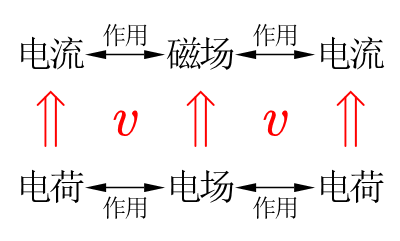
\includegraphics[width=6cm]{image/7-4-3.png}
\caption{磁场与电荷的关系}

\end{wrapfigure}

如何证明磁场是电场的相对论效应. 设想原参考系中只有电场, 那么无论原参考系中的速度$v_x,\,v_y,\,v_z$如何, 受力都不取决于速度大小, 它是:
\[F_x=qE_x\quad ,\quad F_y=qE_y \quad ,\quad  F_z=qE_z\]

根据相对论的力变换公式:
\[F_x'=F_x-\frac{u}{c^2}\cdot\frac{v_yF_y+v_zF_z}{1-\frac{uv_x}{c^2}}\quad ,\quad F_y'=\frac{F_y}{\gamma (1-\frac{uv_x}{c^2})}\quad ,\quad F_z'=\frac{F_z}{\gamma (1-\frac{uv_x}{c^2})}\]

代入原式, 并假设原参考系速度和变换速度相对$c$都是小量, 故新参考系速度可以使用经典的速度叠加:
\[v_x=v_x'+u\quad ,\quad v_y=v_y' \quad ,\quad v_z=v_z'\]

近似到与$v_x',\,v_y',\,v_z'$一阶相关的领头项:

\[F_x'=qE_x-qv_y'\cdot \frac{uE_y}{c^2}-qv_z'\cdot \frac{uE_z}{c^2}\]
\[F_y'=qE_y+qv_x'\cdot \frac{uE_y}{c^2}\]
\[F_z'=qE_z+qv_x'\cdot \frac{uE_z}{c^2}\]

我们如果假设以下\emph{洛伦兹力}(Lorentz force)公式的成立性:
\[\bs{F}=q(\bs{E}+\bs{v}\times \bs{B})\]

它是磁场力分量$\bs{F}_m=q\bs{v}\times \bs{B}$与电场力分量$\bs{F}_e=q\bs{E}$的和. 则受力公式简化为:
\[F_x'=qE_x'+qv_y'B_z'-qv_z'B_y'\]
\[F_y'=qE_y'+qv_z'B_x'-qv_x'B_z'\]
\[F_z'=qE_z'+qv_x'B_y'-qv_y'B_x'\]

对比即知道:
\[B_x'=0\quad ,\quad B_y'=\frac{uE_z}{c^2} \quad ,\quad B_z'=-\frac{uE_x}{c^2}\]

这实际上是:
\[\bs{B}=-\frac{\bs{u}\times \bs{E}}{c^2}\]

如果原参考系是静止点电荷产生的电场, 现在换参考系以后, 点电荷做速度为$-\bs{u}$的匀速直线运动而产生以上磁场, 那么就能推理出, 如果点电荷以速度$\bs{v}$做匀速直线运动, 那么它产生的磁场必然为:
\[\bs{B}=\frac{1}{4\pi \varepsilon_0 c^2}\frac{q\bs{v}\times \bs{e}_r}{r^2}\]

我们从中总结出:
\begin{itemize}
	\item 只有运动的电荷才会受到磁场力.
	\item 只有运动的电荷才产生磁场.
	\item 但是运动与静止具有相对性, 所以电场和磁场的区别就像静止与运动的区别那样是相对的, 合称\emph{电磁场}(electromagneto field).
\end{itemize}

我们还注意到来自理论推导过程中产生的重要公式:

\[\bs{B}=\frac{1}{4\pi \varepsilon_0 c^2}\frac{q\bs{v}\times \bs{e}_r}{r^2}\]
\[\bs{F}=q\bs{v}\times \bs{B}\]

由于推导的近似性这两个式子似乎没有太多说服力. 但是历史上这两个式子是作为实验规律先被总结, 再有麦克斯韦的普遍电磁理论, 最后才是洛伦兹和爱因斯坦对其背后的相对论基础的研究.


\subsection{毕奥-萨伐尔定律}

强调一下本章研究的范围是重要的. 我们暂时只研究\emph{静磁场}(static magnetic field), 其场源为电流, 且其分布不随时间, 从而改变的磁场也不随时间改变. 或者更简单的说, 我们要研究的体系就是上一章建立的稳恒电流体系, 它由不变的电荷产生不变的电场, 不变的电场驱动不变的电流, 现在增加了不变的电流产生不变的磁场这一要素. 上一章的讨论告诉我们这就是要求电流分布是无散的:
\[\nabla \cdot \bs{j}=0\]

如何把微观电荷的运动同宏观的电流$\bs{j},\,I$建立联系? 引言中我们指出来过, 微观运动电荷产生的磁场正比于量:
\[\bs{C}=q\bs{v}\]

这个量被称作\emph{电流元}(current element). 事实上作为微观电荷$q$通常是基本电荷$e$的量级, 从而上述量是一个微元, 即使取物质中一个很小的体积$\ud V$, 其内部包含的所有电荷个数$\ud N$依然未达到宏观量级时, 总的电流元依然是个小量, 记做$\ud\bs{C}$. 我们知道电流密度的定义为:
\[\bs{j}=\rho\bs{v}=nq\bs{v}\]

那么体积产生的总的电流元:
\[\ud \bs{C}=\ud N q\bs{v}=nq\bs{v}\ud V=\bs{j}\ud V=\rho\ud V\cdot\bs{v}\]

称为\emph{体电流元}(volume current element). 同理, 我们可以写出\emph{面电流元}(surface current element)和\emph{线电流元}(curve current element):
\[\ud \bs{C}=\bs{i}\ud A=\sigma\bs{v}\ud A\quad ,\quad \ud \bs{C}=I\ud \bs{l}=\lambda \bs{v}\ud l\]

注意上面线电流元的写法, 由于我们不认为$I$是矢量, 故把电流元的矢量性由线元$\ud \bs{l}$来承载. 这么做的好处之后就能体会到. 我们发现电流元与电荷元形成了对应关系:
\begin{figure}[H]
\centering
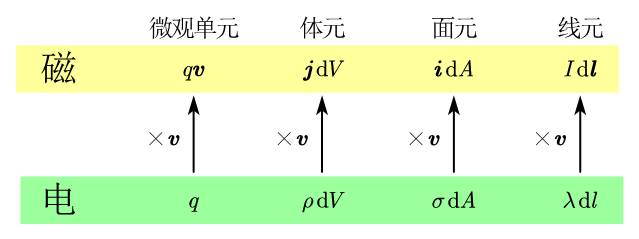
\includegraphics[width=0.6\textwidth]{image/7-4-4.png}
\caption{电荷元与电流元对应}
\end{figure}

\emph{毕奥-萨伐尔定律}(Biot-Savart law)是一个实验定律, 它用于描述真空中两个孤立的电流元之间的相互作用力:
\[\ud \bs{F}_{12}=\frac{\mu_0}{4\pi}\frac{I_2\ud \bs{l}_2\times (I_1\ud \bs{l}_1\times \bs{e}_{12})}{r^2}\]

\begin{wrapfigure}[13]{o}[-10pt]{6cm}
\centering
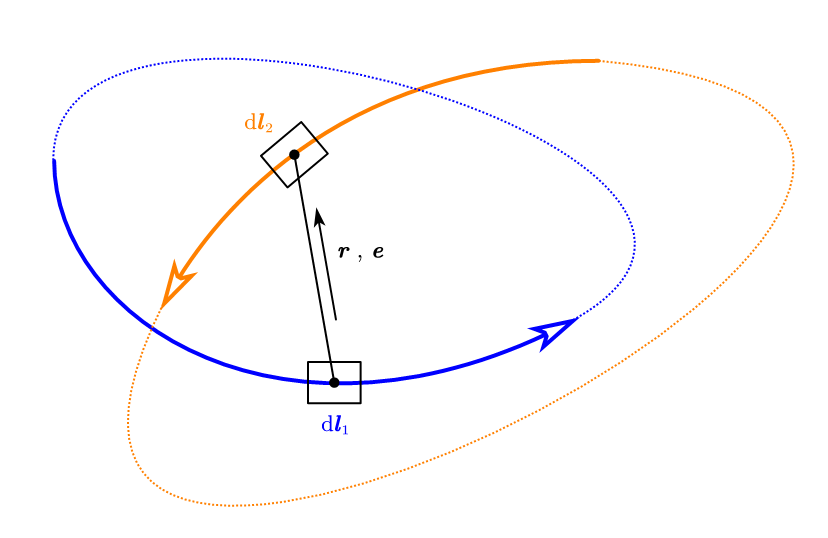
\includegraphics[width=6cm]{image/7-4-5.png}
\caption{电流体系间的相互作用力}
\end{wrapfigure}

其中系数$k_m=\dfrac{\mu_0}{4\pi}\approx 1\times 10^{-7}{\rm H/m}$\footnote{注意, 2019年5月20日之后, 新的国际单位制标准下其值为$1.000\;000\;000\;82(20)\times 10^{-7}{\rm H/m}$, 不再有严格的$\mu_0:=4\pi\times 10^{-7}{\rm H/m}$.}为磁力常数, 而$\mu_0$称作\emph{真空磁导率}(magnetic permeability of vacuum). 事实上:
\[k_e/k_m=c^2\quad \text{或者}\quad c=\frac{1}{\sqrt{\varepsilon_0\mu_0}}\]

$c$是真空中的光速. 这也揭示了电磁理论统一性背后的相对论本质. 我们这里还用到了电感的国际单位亨利, 而磁场的国际单位\emph{特斯拉}(Tesla)与它的关系为:
\[1{\rm H}=1{\rm T\cdot m^2/A}\]

另一个常用的单位来自CGS单位制, 即\emph{高斯}(Gauss), 以纪念这位伟大的数学家在物理学上同样瞩目的贡献. 高斯在历史上被广泛使用, 直至今天也如此, 例如地表地磁场大概就在$0.25-0.60{\rm G}$, 它与特斯拉的换算关系为:
\[1{\rm T}=10000{\rm G}\]

根据场论的精神, 我们将上式拆解为电流产生场的定律和电流在场中受力的公式:
\[\ud \bs{F}_{12}=I_2\ud \bs{l}_2\times \ud \bs{B}_{12}\quad ,\quad \ud \bs{B}_{12}=\frac{\mu_0}{4\pi}\frac{I_1\ud \bs{l}_1\times \bs{e}_{12}}{r^2}\]

\begin{wrapfigure}[13]{o}[-10pt]{6cm}
\centering
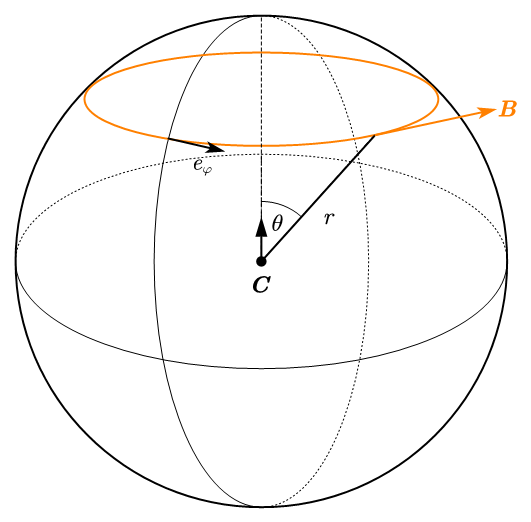
\includegraphics[width=6cm]{image/7-4-6.png}
\caption{电流元产生的磁场}
\end{wrapfigure}
如前所述, 毕奥-萨伐尔定律可以在相对论背景下由库仑定律推出, 故它继承了库仑定律的平方反比和叠加原理的特性. 但是它突出的特点是具有\emph{横向力}(transverse force)的特点: 力的方向与受力物体电流元垂直, 也与另一个只依赖于场源的磁场矢量垂直, 但这个矢量又与场源电流元的方向垂直. 两次叉乘这让力的计算变得比较复杂. 让我们以场源电流元$\bs{C}$为中心, 其方向建立极坐标系, 那么磁场的大小与方向就可以从公式得到:
\[\bs{B}=\kb\frac{C\sin\theta}{r^2}\bs{e}_\varphi \]

磁场符合叠加原理, 例如一个载流线圈, 源点坐标$\bs{r}'$, 场点坐标$\bs{r}$, 记$\bs{R}=\bs{r}-\bs{r}'$, 则其产生的磁场公式为:
\[\bs{B}=\oint \kb\frac{I\ud \bs{l}\times \bs{e}_{\bs{R}}}{R^2}\]

其中$\ud \bs{l}=\ud \bs{r}'$

\begin{figure}[H]
\centering
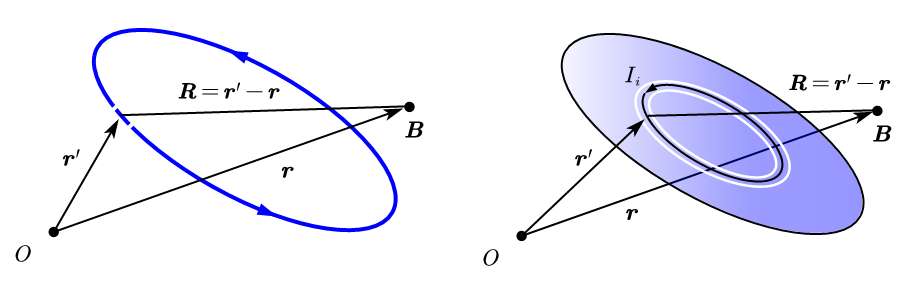
\includegraphics[width=0.8\textwidth]{image/7-4-7.png}
\caption{连续体系产生磁场}
\end{figure}

载流线圈具有非常重要的地位, 任何体电流分布, 只要是有界区域内的稳恒电流, 电流线就必然构成闭合的回路. 那么就一定可以分解为电流圈. 如果用求和的极限表示积分但是暴力地省去极限符号, 此时磁场计算方法为:
\[\bs{B}=\int\limits_{V'} \kb\frac{\bs{j}\times \bs{e}_{\bs{R}}}{R^2}\ud V=\sum_i \oint \kb\frac{I_i\ud \bs{l}_i\times \bs{e}_{\bs{R}}}{R^2}\]

而一个线圈或一个体电流分布在外磁场中的受力为:
\[\bs{F}=\oint I\ud\bs{l}\times \bs{B}\]
\[\bs{F}=\sum_i I_i\ud\bs{l}_i\times \bs{B}\]

在稳恒电流情况下, 讨论一个电流元产生的磁场是没有意义的, 因为空间的磁场必然是整个体系产生的磁场的叠加, 从而单个电流元的磁场并不具有可观测的意义, 除非电流可以独立的被操控以改变. 而讨论一个电流体系各个部分受到的作用力时, 尤其是一个电流线圈受到的作用力时, 区分内力和外力就变得尤其重要. 我们发现, 两个电流元之间的相互作用力之和:
\[\ud \bs{F}_{12}+\ud \bs{F}_{21}=\frac{\mu_0}{4\pi}\frac{I_2\ud \bs{l}_2\times (I_1\ud \bs{l}_1\times \bs{e}_{12})}{r^2}+\frac{\mu_0}{4\pi}\frac{I_1\ud \bs{l}_1\times (I_2\ud \bs{l}_2\times \bs{e}_{21})}{r^2}\]

根据三重矢积公式$\bs{A}\times(\bs{B}\times\bs{C})=(\bs{A}\cdot\bs{C})\bs{B}+(\bs{A}\cdot\bs{B})\bs{C}$, $\bs{e}_{12}=-\bs{e}_{21}$. 得到:
\[\ud \bs{F}_{12}+\ud \bs{F}_{21}=-\kb \frac{(I_1\ud \bs{l}_1\times I_2\ud \bs{l}_2)\times \bs{e}_{12}}{r^2}\]

一般来说不总为零, 可见朴素的牛顿第三定律在静磁场情况下失效了. 我们不得不把$\ud\bs{F}_{12},\,\ud \bs{F}_{21}$不再视作相互作用力, 而是需要通过场作为媒介. 事实上两个运动电荷之间的磁场力是在作为电场力的相对论修正, 从相对论的根本原理上, 相互作用传递速度的有限性导致力的传播被推迟, 原则上也不可能符合牛顿第三定律.

但是如果我们计算两个线圈之间的相互作用力之和:
\begin{align*}
\delta\bs{F}&=\oint\limits_1\oint\limits_2\ud \bs{F}_{12}+\oint\limits_2\oint\limits_1\ud \bs{F}_{21}\\
&=\frac{\mu_0I_1I_2}{4\pi}\left(\oint\limits_1\oint\limits_2\frac{(\bs{r}_2-\bs{r}_1)\cdot\ud(\bs{r}_2-\bs{r}_1)}{|\bs{r}_2-\bs{r}_1|^3}\ud\bs{r}_1+\oint\limits_2\oint\limits_1\frac{(\bs{r}_1-\bs{r}_2)\cdot\ud(\bs{r}_1-\bs{r}_2)}{|\bs{r}_1-\bs{r}_2|^3}\ud\bs{r}_2\right)
\end{align*}

但是:
\[\nabla_2 \frac{1}{|\bs{r}_2-\bs{r}_1|}=-\frac{\bs{r}_2-\bs{r}_1}{|\bs{r}_2-\bs{r}_1|^3}\quad\Rightarrow\quad \oint\limits_2\frac{(\bs{r}_2-\bs{r}_1)\cdot\ud(\bs{r}_2-\bs{r}_1)}{|\bs{r}_2-\bs{r}_1|^3}=0\]
\[\nabla_1 \frac{1}{|\bs{r}_1-\bs{r}_2|}=-\frac{\bs{r}_1-\bs{r}_2}{|\bs{r}_1-\bs{r}_2|^3}\quad\Rightarrow\quad \oint\limits_1\frac{(\bs{r}_1-\bs{r}_2)\cdot\ud(\bs{r}_1-\bs{r}_2)}{|\bs{r}_1-\bs{r}_2|^3}=0\]

从而得到:
\[\delta\bs{F}=0\]

或者说, 一个静磁体系内部两部分之间的相互作用力之和必然为零. 这个结果其实也是空间平移对称性的必然结果. 而空间旋转对称性则给出, 任意选取$O$点计算各个电流元受力对$O$的力矩, 总和必然为零. 或者说两个线圈之间的作用力与作用力矩之间必然符合牛顿第三定律. 其证明在此不再赘述. 这样我们就证明了此前给出的理论公式与牛顿第三定律之间是自洽的, 无散的电流体系下牛顿第三定律依然成立, 尽管表面上电流元的毕奥萨伐尔定律与牛顿第三定律有冲突.

更有甚者, 我们指出, 根据麦克斯韦方程的协变性, 即使是微观电荷做相对论性运动, 只要是稳恒电流体系, 那么毕奥萨伐尔定律可以作为一个推论而具有普适性. 而对于非稳恒体系, 后面我们将会证明, 磁场此时并不能简单地由电流确定而依赖于电场的变化率, 甚至它成为了自由存在的物质形式而摆脱了电荷造成的任何约束.




\section{两个定律与矢势}

\subsection{磁场环路定律}

\begin{itemize}

\item 磁场环路定律, 又名安培环路定律:
\[\oint\limits_{\partial S}\bs{B}\cdot \ud \bs{l}=\mu_0 \int\limits_S\bs{j}\cdot \ud \bs{S}\]
\[\nabla\times \bs{B}=\mu_0 \bs{j}\]

\item 
\end{itemize}

\subsection{矢势与磁场高斯定律}

\begin{itemize}

\item 对电流元引入以下矢量场是方便的:
\[\bs{A}=\frac{\mu_0}{4\pi}\frac{\bs{j}\ud V}{r}\]

这是因为计算可得, 这直接导致了:
\[\bs{B}=\frac{\mu_0}{4\pi}\frac{\bs{j}\ud V\times \bs{e}_r}{r^2}=\nabla\times \bs{A}\]

这个矢量称作\emph{磁矢势}(magnetic vector potential).

\item 由于叠加原理, 一个电流分布体系的磁矢势和磁场应当为:
\[\bs{A}=\int\limits_V \frac{\mu_0}{4\pi}\frac{\bs{j}\ud V}{r}\quad ,\quad \bs{B}=\int\limits_V \frac{\mu_0}{4\pi}\frac{\bs{j}\ud V\times \bs{e}_r}{r^2}\]

同样地将满足:
\[\bs{B}=\nabla\times \bs{A}\]

\item 以上旋度关系写成积分形式意味着一种计算磁通量的特殊方法:
\[\Phi=\oint\limits_{\partial S} \bs{A}\cdot \ud \bs{l}=\int\limits_S\bs{B}\cdot \ud \bs{S}\]


\item 对于无边界的闭合曲面, 上式直接证明了磁场高斯定律:
\[\oint\limits_{\partial V}\bs{B}\cdot \ud \bs{S}=0\]
\[\nabla\cdot \bs{B}=0\]

\item 可以设想存在可以像点电荷产生电场那样的方式产生磁场的物质, 称作\emph{磁单极子`}(magnetic monopole), 从而可以产生不为零的净\emph{磁荷}(magnetic charge), 事实证明这样的物质至今都未曾找到, 从而相伴的磁场形式也仅仅存在与理论中. 但是, 总磁荷为零的体系: \emph{磁偶极子}(magnetic dipole), 不仅仅是纯粹的理论模型, 后面可以发现线圈产生的磁场与磁偶极子是相似的.
\end{itemize}


\section{电流体系}

\subsection{磁偶极子}

\begin{itemize}
\item \emph{磁偶极子}(magnetic dipole)模型一般不指由正负磁单极子构成的体系, 和电偶极子类似, 它也来自矢势与磁场计算过程中的多极展开, 由于需要用到较深的张量知识, 在此仅仅给出展开的结果:
\[\bs{m}=\frac{1}{2}\int\limits_V \bs{r}\times \bs{j}\ud V\quad ,\quad \bs{A}=\frac{\mu_0}{4\pi}\frac{\bs{m}\times \bs{e}_r}{r^2}\quad ,\quad B_r=\frac{\mu_0}{4\pi}\frac{2m\cos\theta }{r^3}\quad ,\quad B_\theta=\frac{\mu_0}{4\pi}\frac{m\sin\theta }{r^3}\]

其中$\bs{m}$称作\emph{磁矩}(magnetic moment), 任何情况下这都会是一个电流体系激发的磁场的领头项, 因为磁单极子不存在, 类似点电荷产生平方反比的电场那样的磁荷项, 由于磁高斯定律, 永远是不可能的.

\item 一个线圈, 面矢量为$\bs{S}$, 它的磁矩, 由于以下积分公式:
\[\bs{S}=\frac{1}{2}\oint\limits_{\partial S}\bs{r}\times \ud \bs{r}\]

可以发现:
\[\bs{m}=\frac{1}{2}\int\limits_V \bs{r}\times I \ud \bs{l}=I\bs{S}\]

如果考虑$I\to \infty, S\to 0$的模型, 就构成了\emph{点磁偶极子}(point dipole).

\item 磁偶极子的磁势能, 受力与力矩:
\[V=-\bs{m}\cdot \bs{B}\quad ,\quad \bs{F}=\bs{m}\cdot \nabla\bs{B}\quad ,\quad \bs{M}=\bs{m}\times \bs{B}\]

\end{itemize}

\subsection{磁化强度}

\begin{itemize}
\item \emph{磁化强度}(magnetization):
\[\bs{M}=n\bs{m}\]

\item 磁化强度造成的体电流与面电流分布:
\[\bs{j}_M=\nabla\times \bs{M}\quad ,\quad \bs{i}_M=\bs{M}\times \bs{n}\]


\end{itemize}

\subsection{若干对称体系的磁场}

\begin{itemize}
\item 无限长载流直线:
\[\bs{A}=-\frac{\mu_0 I}{2\pi}\ln r\quad ,\quad \bs{B}=\frac{\mu_0 I}{2\pi r}\bs{e}_\varphi\]

\begin{figure}[H]
\centering
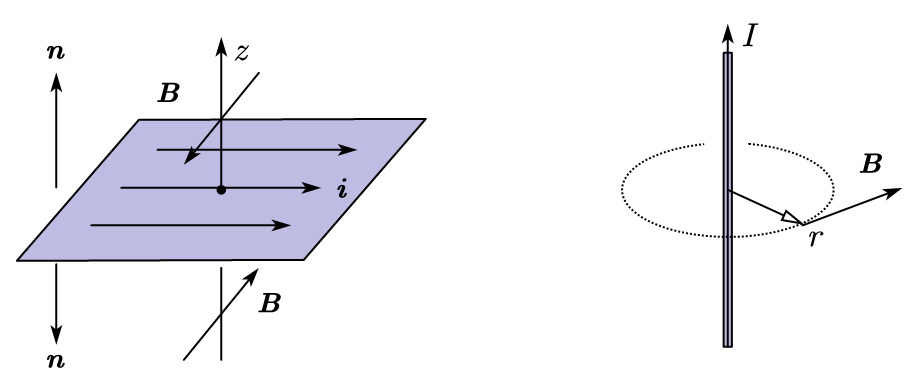
\includegraphics[width=0.7\textwidth]{image/7-4-1.png}
\caption{无限大平面与无限长直线}\label{fig7-4-1}
\end{figure}

\item 无限大载流平面:
\[\bs{B}=\frac{1}{2}\mu_0\bs{i}\times \bs{n}\]

\item 圆环: 半径为$R$的标准载流线圈轴线上磁场:
\[\bs{B}=\frac{\mu_0IR}{2(R^2+z^2)^{\frac{3}{2}}}\bs{e}_z\]

该处的径向场强可以由磁高斯定理确定:
\[\frac{1}{2}\frac{\ud B_r}{\ud r}+\frac{\ud B_z}{\ud z}=0\quad \Rightarrow \quad B_r\approx -\frac{3\mu_0IRzr}{(R^2+z^2)^{\frac{5}{2}}}\]

\item 无限长密绕螺线管: 无论其横截面形状, 总是有:
\[B=\mu_0 i=\mu_0 nI=\frac{\mu_0 NI}{l}\]
\end{itemize}


\npg{-2cm}

\section{磁介质与磁能}

\subsection{微观角度理解磁化}

\begin{itemize}
\item 分子的固有磁矩: 电子自旋磁矩+电子轨道磁矩.
\item 如果分子具有固有磁矩, 那么按照热力学规律发生取向磁化: 磁矩倾向于取与外磁场相同的方向, 宏观上产生\emph{顺磁性}(paramagnetism). 类似于电介质的极化, 微观上顺磁磁化规律可以写作:
\[\bar{\bs{\mu}}=\alpha \bs{B}\]
\item 电子的磁矩与角动量的比称为\emph{旋磁比}(gyromagnetic ratio), 轨道旋磁比与自旋旋磁比分别为:
\[\gamma_L=-\frac{e}{2m_e}\quad ,\quad \gamma_S=-\frac{e}{m_e}\]

角动量量子化理论告诉我们, $z$方向上电子轨道与自旋角动量只能为:
\[L_z=\pm n\hbar \quad ,\quad  S_z=\pm \frac{\hbar}{2}\]

故$z$方向上的磁矩的单位就是著名的\emph{玻尔磁子}(Bohr magneton):
\[\mu_B=\frac{e\hbar}{2m_e}=0.00579{\rm meV/T}\]

事实上由于自旋-轨道耦合, 分子磁矩可以是玻尔磁子的分数倍.

\item 原子核也有磁矩, 显然由于质子质量比质子质量大三个量级, 故根据旋磁比算法, 其磁矩也小三个量级. 虽然对分子磁矩和宏观磁化几乎没有贡献, 但是利用在磁场下形成的各个能级间跃迁吸收发射电磁辐射的原理可以造成\emph{核磁共振}(nuclear magnetic resonance)现象.

\item 如果分子的固有磁矩为零, 那么在外磁场下会产生一个与外磁场反向的磁矩, 宏观上造成\emph{抗磁性}(diamagnetism). 从微观来看似乎与电介质极化的方向相反, 但是从宏观效果上却与电介质削弱电场的效果相同, 这是电与磁固有的区别导致的.

\item 抗磁性的微观起源为电子轨道运动的\emph{拉莫尔进动}(Larmor precession). 由轨道运动产生的力矩, 角动量, 磁矩三者关系可得:
\[\bs{M}=\bs{\mu}\times \bs{B}\quad ,\quad  \bs{\mu}=\gamma \bs{L}\quad ,\quad  \frac{\ud}{\ud t}\bs{L}=\bs{M}\]
\[\Rightarrow \quad  \frac{\ud}{\ud t}\bs{L}=-\gamma \bs{B}\times \bs{L}=\frac{e\bs{B}}{2m}\times \bs{L}\]

故在运动学上, 电子将以以下角速度发生进动:
\[\bs{\Omega}=\frac{e}{2m}\bs{B}\]

电子原来的轨道运动半径如果按照玻尔半径$a_0$估计, 而角动量量级为$\hbar$, 那么现在附加的角速度与原来的角速度的比为:
\[\Omega/\omega\sim\frac{ea_0^2}{2\hbar}B\]

故产生的磁矩与原来的玻尔磁子的比值的量级也与之相当, 得到磁矩的量级为:
\[\bar{\bs{\mu}}\sim-\frac{e^2a_0^2	}{4m}\bs{B}\]

系数便是抗磁性磁化的分子磁化率的量级, 它一般比顺磁性磁化要小一到两个量级.

\item 有一些金属, 或者特殊的金属化合物具有独特的\emph{铁磁性}(ferromagnetism), 微观上它们由介观的包含大量原子的\emph{磁畴}(magnetic domains)构成. 每一个磁畴由于单元之间的关联已经超过了热力学的涨落而成为了决定性的因素, 使得所有电子的自旋几乎都严格指向同一个方向, 磁化达到饱和. 而材料的磁化过程其实是不同的磁畴在外磁场下的转向. 它的磁化率将远远大于简单的顺磁和抗磁磁化. 而且体现出非线性和历史相关性.


\end{itemize}

\subsection{宏观角度理解磁化}

\begin{itemize}
\item 出于$\bs{B}$和$\bs{M}$的旋度分别为总电流密度和磁化电流密度, 引入\emph{磁场强度}(magnetic field strength)以区别于以往一贯描述磁场的$\bs{B}$, 一般可区别称作\emph{磁通密度}(magnetic flux density):
\[\bs{H}=\frac{\bs{B}}{\mu_0}-\bs{M}\]

这样这个矢量的旋度就只取决于外电流:
\[\nabla\times \bs{H}=\bs{j}_f\]

\item 在顺磁或铁磁的柱状介质外绕制密绕螺线管, 那么没有介质时其磁通密度为:
\[B_0=\mu_0 i\]

那么, 由于此时加入介质时磁化电流不影响$\bs{H}$的计算, 故磁场强度为:
\[H=\frac{B_0}{\mu_0}=i\]

但是磁化电流的存在将产生一个与原磁场同向的附加磁场, 使得介质内部的磁场变大, 那么定义此时磁场与原磁场的比值为\emph{相对磁导率}(relative magnetic permeability):
\[B/B_0=\mu_r\]

那么把绝对磁导率定义为$\mu=\mu_r\mu_0$, 就有以下关系式:
\[B=\mu H=\mu i\]

\[M=(\mu_r-1)H=\chi_m H\]

其中$\chi_m$就是宏观的\emph{磁化率}(magnetic susceptibility). 对于抗磁性物质, 其值是小于零的.


\end{itemize}

\subsection{磁场能量}

磁场体系的能量的计算方法可以证明可以有用电流与矢势和用能量密度两种计算方法:
\[I=\frac{1}{2}\int \bs{j}\cdot\bs{A}\ud V=\int \frac{1}{2\mu_0}	\bs{B}^2\ud V\]

同样地, 两个体系同时存在时, 体系将产生自能与相互作用能. 如两个电感元件如果之间存在互感, 那么其总能量应当为:
\[E=\frac{1}{2}L_1I_1^2+\frac{1}{2}L_2I_2^2+ MI_1I_2\]

如果存在介质, 其能量密度需要加上磁化带来的能量, 能量密度变为:
\[w=\frac{1}{2\mu}	\bs{B}^2=\frac{1}{2}\mu \bs{H}^2 =\frac{1}{2}	\bs{B}\cdot \bs{H}\]

%\section{超导简介}
